\chapter{Proposta}

Neste capítulo, em continuidade à problemática levantada, será apresentada a proposta de solução que é o objeto deste trabalho.

\section{Funcionamento}
O sistema proposto para a automação do jogo Contexto opera de forma integrada, simulando um jogador humano por meio de um ciclo de inferência semântica. O funcionamento é orquestrado pela classe \textit{ContextoSolver}, que gerencia a lógica de inferência e é desacoplada da interface do jogo. 

Uma vez que a automação é iniciada, o ContextoSolver é inicializado com um modelo de word embedding pré-treinado podendo ser GloVe, Word2Vec ou FastText carregado pelo Gensim. O processo de resolução se começa com a exploração, na qual o sistema submete \textit{seed words} (palavras semente) para obter um \textit{feedback} inicial do jogo e extrair o \textit{rank} de similaridade retornado.

Com esse feedback, o ContextoSolver analisa o rank e armazena o resultado no histórico. A heurística de seleção utiliza o Gensim para calcular a similaridade vetorial e gerar novas palavras candidatas que sejam semanticamente próximas das melhores tentativas anteriores.

A Figura~\ref{fig:FluxoSistema} apresenta o diagrama de sequência para facilitar a compreensão.

\begin{figure}[h!]
    \centering
    
    \caption{Diagrama de Sequência}
    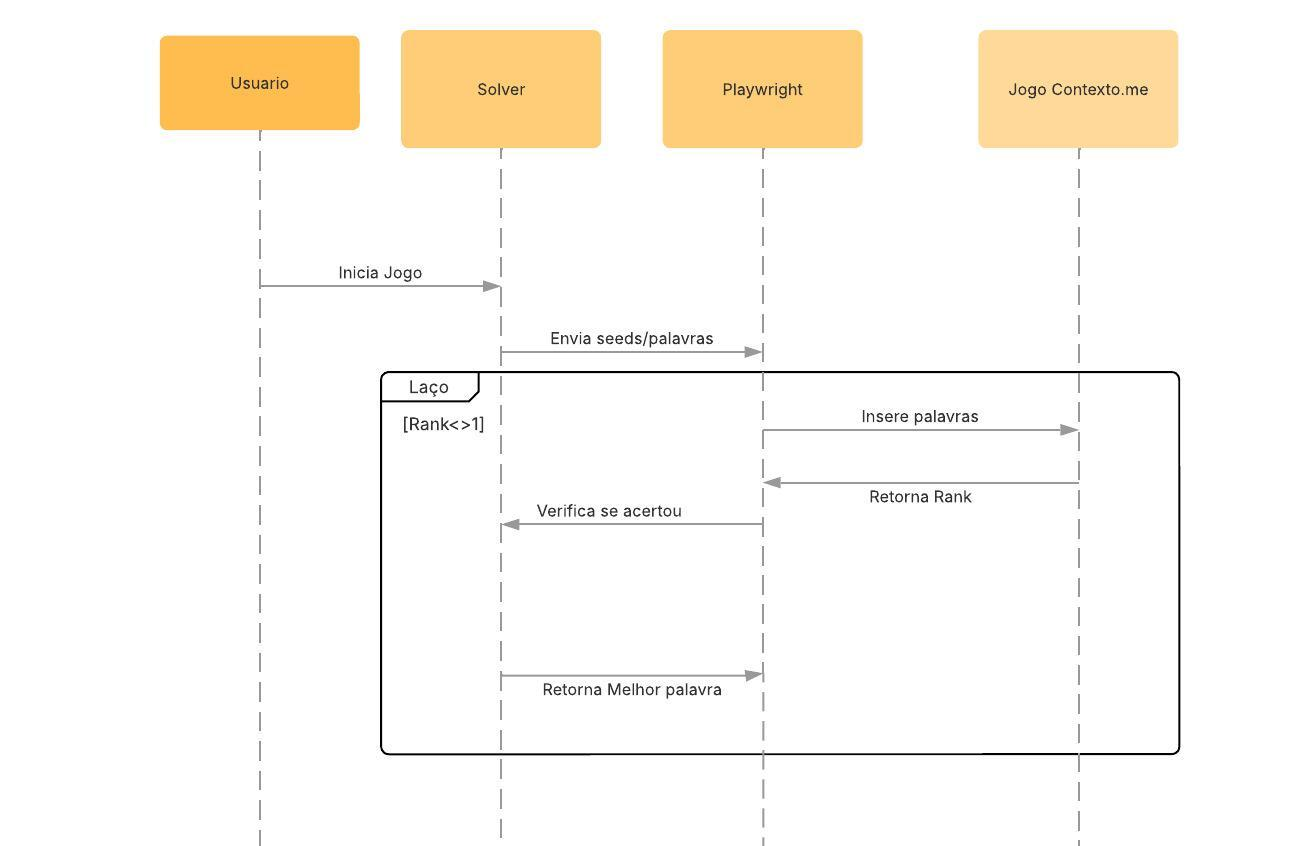
\includegraphics[width=1\textwidth]{figs/Diagrama.jpeg}
    \label{fig:FluxoSistema}
    
    Fonte: Elaborado pelos autores
\end{figure}

Este ciclo de tentativa, coleta de feedback e análise é repetido. Quando o sistema atinge um rank suficientemente bom, ele entra em modo de otimização utilizando um modelo de Regressão Ridge, que é treinado em tempo real com o histórico de tentativas para prever quais palavras do vocabulário têm maior probabilidade de estarem próximas da resposta.

O sistema então passa a escolher palavras com base nas previsões desse modelo, refinando a busca.
O processo continua até que o rank 1 seja alcançado, ou o limite de tentativas seja atingido. 

A Figura ~\ref{fig:Diagrama} apresenta o fluxograma da lógica de execução do sistema para facilitar a compreensão.

\begin{figure}[H]
    \centering
    
    \caption{Fluxograma da Lógica de Execução do Sistema}
    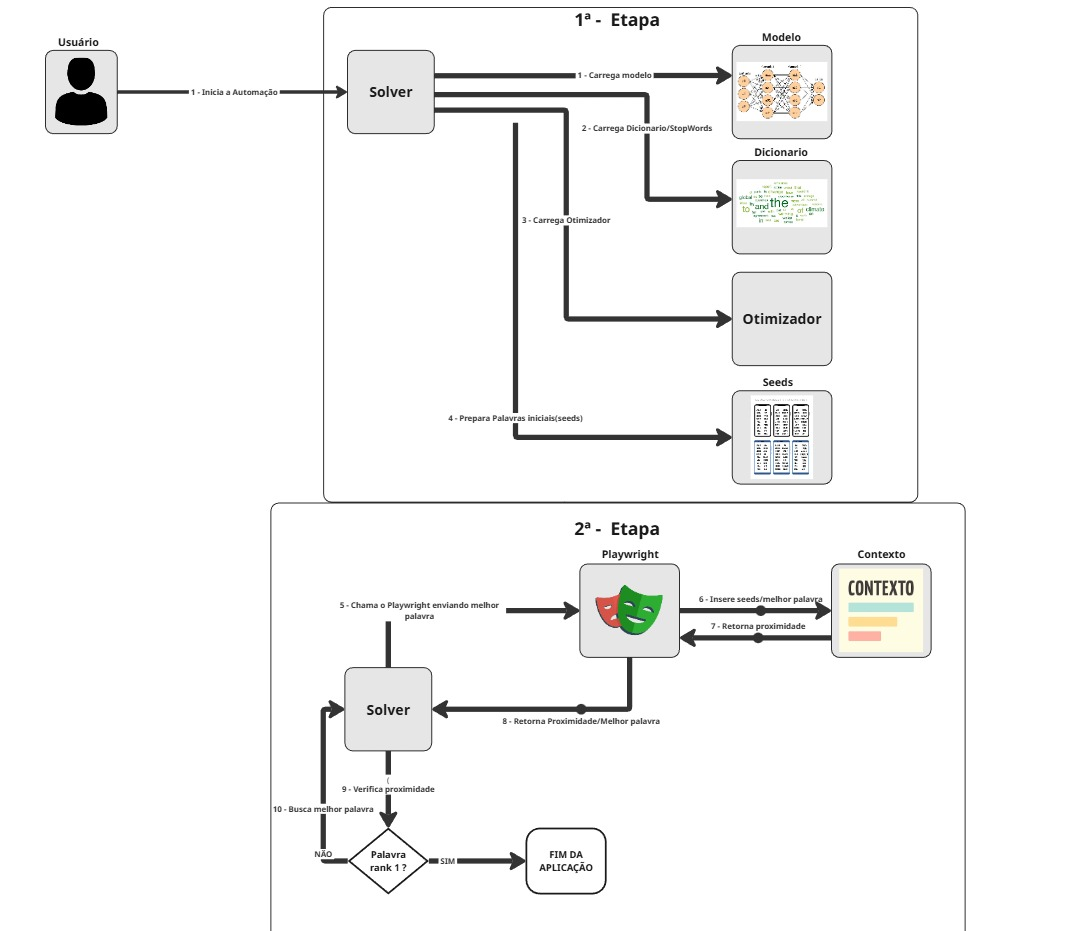
\includegraphics[width=1\textwidth]{figs/diagramadefluxo.jpg}
    \label{fig:Diagrama}
    
    Fonte: Elaborado pelos autores
\end{figure}

\section{Arquitetura}
O sistema proposto segue uma arquitetura modular dividida em três componentes principais que trabalham de forma integrada: a interface com o jogo, o processamento semântico e a lógica de controle.

A interface com o jogo é implementada utilizando o Playwright, encapsulada na classe \textit{ContextoOnline}. Esse módulo é responsável por acessar a página do jogo, preencher automaticamente as tentativas de palavras, ler o feedback e detectar quando a palavra correta é encontrada. A implementação gerencia \textit{timeouts} e sincronizações para garantir a estabilidade da automação.

O processamento semântico constitui o núcleo inteligente do sistema, empregando a biblioteca Gensim para gerenciar os word embeddings no formato \textit{KeyedVectors}. Este componente permite comparar diferentes modelos pré-treinados (GloVe, Word2Vec, FastText) e utiliza \textit{Numpy} para realizar as operações matemáticas de similaridade e aritmética vetorial, essenciais para a geração de novas palavras candidatas.

A lógica de controle, implementada em Python na classe ContextoSolver, orquestra a comunicação entre os módulos e gerencia o fluxo de execução. Este componente envia as palavras geradas para a interface, processa os ranks recebidos e atualiza o estado do jogo (histórico de palavras, melhores tentativas). A classe implementa a heurística de seleção de palavras, alternando entre o modo de "exploração", baseado em similaridade vetorial, e o modo de "otimização", usando Regressão Ridge.

\section{Detalhes de Implementação}
A implementação do sistema utilizou Python 3.12, integrando as bibliotecas Playwright para automação do navegador, Gensim para o processamento dos embeddings, Numpy para computação científica e \textit{scikit-learn} para o modelo de Regressão Ridge.

Foram utilizados modelos de word embedding pré-treinados para o português, especificamente os modelos de 300 dimensões disponibilizados pelo Núcleo Interinstitucional de Linguística Computacional (NILC) em \citeonline{hartmann-etal-2017-portuguese}.

\section{Estrutura e Funções Desenvolvidas}
Esta seção tem como objetivo explicar as principais classes e métodos desenvolvidos para
implementar a proposta apresentada neste estudo, fornecendo uma análise detalhada
de como as funções são estruturadas e implementadas. O objetivo é proporcionar uma
compreensão abrangente dos equipamentos técnicos utilizados, destacando sua relevância
e eficácia na realização da análise e na obtenção dos resultados desejados nesta tese.

\subsection{ContextoSolver}
O Código \ref{lst:contexto-solver} apresenta a classe ContextoSolver, responsável por controlar o fluxo completo de automação. Essa classe orquestra a comunicação entre os modelos semânticos e o jogo, gerando tentativas de palavras, analisando o retorno de similaridade e refinando as jogadas subsequentes.

\begin{lstlisting}[
    language=Python,
    caption=Classe ContextoSolver,
    label={lst:contexto-solver}
]
class ContextoSolver:
    def __init__(
        self,
        model: KeyedVectors,
        query_function: Callable,
        optimization_rank_limit: int = 100,
        max_vocab: int = 150_000,
        random_state: int = 42
    ):
        self.model = model
        self.query_function = query_function
        self.optimization_rank_limit = optimization_rank_limit
        self.rng = random.Random(random_state)
        
        with open("dicionario_ptbr.txt", "r", encoding="utf-8") as f:
            self.portuguese_dictionary = {line.strip().lower() for line in f}
        self.stopwords = set(nltk.corpus.stopwords.words("portuguese"))
        self.stemmer = nltk.stem.RSLPStemmer()

        print("Filtrando vocabulário com base no dicionário (pode levar um momento)...")
        base_vocab = model.index_to_key[:max_vocab]
        self.vocab = {w for w in base_vocab if self._is_valid_word(w)}
        print(f"Vocabulário filtrado para {len(self.vocab)} palavras válidas.")

        default_seeds = ["animal", "objeto", "lugar", "corpo", "natureza", "alimento", "ferramenta", "sentimento"]
        self.seed_words = [w for w in default_seeds if w in self.vocab]

        self.guessed = set()
        self.history = list()
        self.best_words = list()
        self.best_rank = float("inf")

        self.reg = Ridge(alpha=0.5, random_state=random_state)
        self.X_obs = list()
        self.y_obs = list()
        self._fitted = False 
        self.optimization_mode = False

    def _observe_and_learn(self, word: str, rank: int):
        ...

    def _get_candidates_from_history(self) -> set:
        ...

    def _choose_next(self) -> str:
        ...

    def solve(self, max_attempts: int = 200, verbose: bool = True) -> list:
        for attempt in range(1, max_attempts + 1):
            current = self._choose_next()
            if current in self.guessed: continue

            rank = self.query_function(current)
            if rank is None:
                self.guessed.add(self._apply_lemmatizer(current))
                continue
            
            self._observe_and_learn(current, rank)
            
            if verbose:
                mode = "OPTIMIZE" if self.optimization_mode else "EXPLORE"
                print(f"Tentativa {attempt:03d} [{mode}]: {current:<15} -> rank {rank:<5} (Melhor: {self.best_rank})")

            if rank == 1:
                print(f"Descoberta em {attempt} tentativas: {current}")
                break
        
        if self.best_rank != 1:
            print(f"Não encontrou a palavra. Melhor tentativa: '{self.best_words[0][0]}' (rank {self.best_words[0][1]})")

        return self.history
    
    def _is_valid_word(self, w: str) -> bool:
        """
        Verifica se a palavra é válida:
        1. Apenas letras.
        2. Minúscula.
        3. Não é uma stopword.
        4. Tem mais de 2 letras.
        5. Existe no dicionário pt-br.
        """
        return (
            w.isalpha() and
            w.islower() and
            w not in self.stopwords and
            len(w) > 2 and
            w in self.portuguese_dictionary
        )
    
    def _apply_stemmer(self, w: str) -> str:
        """Aplica a stemização na palavra."""
        return self.stemmer.stem(w)
    
    def _apply_lemmatizer(self, w: str) -> str:
        """Aplica a lematização na palavra."""
        return lemmatize(w, lang="pt")
    
    def _is_new(self, w: str) -> bool:
        return self._apply_lemmatizer(w) not in self.guessed
\end{lstlisting}

A classe recebe como entrada um modelo pré-treinado de word embeddings no formato KeyedVectors da biblioteca Gensim, estrutura essencial para um mapeamento entre chaves e vetores — sendo a chave, neste contexto, uma palavra.

Inicialmente, o vocabulário do modelo é submetido a um processo de filtragem, que elimina termos inválidos, \textit{stopwords} e palavras não reconhecidas no dicionário da língua portuguesa, garantindo que apenas vocábulos adequados sejam considerados durante o processo de busca. Além disso, é aplicada a lematização das palavras por meio da biblioteca \textit{Simplemma}, com o intuito de normalizar as diferentes flexões de um mesmo termo, evitando repetições desnecessárias nas tentativas.

O impacto dessas etapas de pré-processamento é determinante para a eficácia do algoritmo. A remoção de \textit{stopwords} atua na mitigação de ruído vetorial, impedindo que termos de alta frequência e baixo conteúdo semântico (como preposições e artigos) influenciem erroneamente o cálculo de similaridade, o que poderia desviar a busca do contexto central da palavra secreta.

Paralelamente, a lematização desempenha um papel crucial na redução da dimensionalidade do espaço de busca. Ao condensar plurais, gêneros e conjugações verbais em suas formas canônicas, o algoritmo evita tentativas redundantes, como testar "correr", "correndo" e "correu" sequencialmente, o que resulta em uma convergência mais rápida para a solução e em uma economia significativa de recursos computacionais durante as iterações.

O funcionamento interno do ContextoSolver baseia-se em um ciclo iterativo de exploração e otimização. Durante a exploração, o algoritmo seleciona palavras candidatas próximas às melhores tentativas já realizadas, com base na similaridade vetorial calculada pelo modelo de embeddings.

Quando o desempenho atinge um determinado limiar, o sistema passa a operar em modo de otimização, empregando um modelo de Regressão Ridge para estimar a proximidade semântica entre novas palavras e a solução esperada. Esse modelo supervisionado é continuamente ajustado com base no histórico de respostas, de modo a aprimorar a seleção dos candidatos mais promissores.

A função principal, \textit{solve}, é responsável por coordenar todo o processo de resolução, controlando a escolha das palavras, a interação com o jogo, a coleta dos ranks retornados e o aprendizado incremental do modelo. Essa função mantém o registro das tentativas e aplica os critérios de parada quando a palavra correta é identificada ou o número máximo de tentativas é atingido.

\subsection{Prepare Embedding}
A unidade presente no Código \ref{lst:prepare-embedding} tem como objetivo padronizar o carregamento de modelos de embeddings disponibilizados na plataforma Hugging Face\footnote{\url{https://huggingface.co/}}, convertendo-os para o formato KeyedVectors, o que facilita tanto a utilização quanto a comparação entre diferentes modelos de representações semânticas.

\begin{lstlisting}[
    language=Python,
    caption=Arquivo prepare\_embedding.py,
    label={lst:prepare-embedding}
]
import numpy as np
from gensim.models import KeyedVectors
from huggingface_hub import hf_hub_download
from safetensors.numpy import load_file

def load_huggingface_to_gensim(repo_id: str) -> KeyedVectors:
    path = hf_hub_download(repo_id, "embeddings.safetensors")

    vectors = load_file(path)["embeddings"]
    
    vocab_path = hf_hub_download(repo_id, "vocab.txt")
    
    with open(vocab_path, "r", encoding="utf-8") as f:
        vocab = [w.strip() for w in f]

    kv = KeyedVectors(vector_size=vectors.shape[1])
    kv.add_vectors(vocab, np.array(vectors, dtype=np.float32))
    return kv
\end{lstlisting}

A função realiza o download automático dos artefatos do repositório especificado no Hugging Face e, em seguida, instancia um objeto KeyedVectors dimensionado de acordo com a quantidade de dimensões dos vetores carregados. Após o carregamento, o algoritmo realiza a inserção dos pares chave–vetor, garantindo compatibilidade e eficiência no processamento.

O resultado é um modelo Gensim plenamente funcional, capaz de preservar a correspondência entre termos e suas representações vetoriais, permitindo sua integração direta a classe ContextoSolver.

\section{Modelos Utilizados}
Para o processamento das palavras e o cálculo das similaridades semânticas, foram empregados três modelos de word embeddings previamente treinados para a língua portuguesa, a saber: Word2Vec, FastText e GloVe. Esses modelos foram escolhidos por representarem abordagens consolidadas e complementares no processamento de linguagem natural, permitindo uma análise comparativa quanto à sua eficiência na tarefa de resolução do Contexto.

Os modelos de word embeddings utilizados nesta pesquisa baseiam-se no trabalho de \citeonline{hartmann-etal-2017-portuguese}, desenvolvido pelo NILC. Os autores disponibilizaram 31 arquiteturas treinadas sobre um corpus robusto, composto por mais de 1,3 bilhão de \textit{tokens} e 3,8 milhões de tipos de palavras, abrangendo o português brasileiro e europeu. A heterogeneidade das fontes — que incluem a Wikipédia, portais de notícias, obras literárias e textos acadêmicos — desempenha um papel crucial no desempenho da solução proposta neste trabalho.

Essa diversidade assegura que as representações vetoriais capturem nuances semânticas complexas, garantindo que a proximidade calculada entre os vetores reflita, com alta fidelidade, o uso real e cotidiano da língua, o que é determinante para a eficácia das heurísticas de busca empregadas.

\section{Integração com o Playwright}
A classe ContextoOnline, demostrada no Código \ref{lst:contexto-online}, desempenha um papel importante no funcionamento do sistema, atuando como um módulo intermediário entre o componente solucionador e o ambiente interativo. Seu propósito é estabelecer a comunicação entre o algoritmo solucionador e a interface do jogo Contexto.

Através da biblioteca Playwright, o algoritmo realiza o envio das palavras sugeridas pelo ContextoSolver diretamente na interface web do jogo, reproduzindo as ações humanas de digitação e envio. Em seguida, coleta e extrai os resultados retornados, como ranking e outros indicadores exibidos na página.

\begin{lstlisting}[
    language=Python,
    caption= Classe ContextoOnline,
    label={lst:contexto-online}
]
class ContextoOnline:
    def __init__(self, headless: bool = True):
        """
        headless: True roda sem janela
        """
        self.headless = headless
        self._play = None
        self._browser = None
        self._page = None

    def start(self):
        self._play = sync_playwright().start()
        self._browser = self._play.chromium.launch(headless=self.headless)
        self._page = self._browser.new_page()
        self._page.goto("https://contexto.me/pt/", wait_until="domcontentloaded", timeout=60000)
        return self
    
    def close(self):
        if self._browser:
            self._browser.close()

        if self._play:
            self._play.stop()

    def query(self, guess: str) -> int | None:
        """
        Envia 'guess' e retorna o rank (int). Se não conseguir ler, retorna None.
        Corrigido para ler a PRIMEIRA linha (a mais recente) e extrair números com milhares/sufixos.
        """
        try:
            prev_count = len(self._page.query_selector_all("div.row"))
        except Exception:
            prev_count = 0

        print(f"Enviando chute: {guess}")
        self._page.fill("input[type='text'], input", guess)
        self._page.keyboard.press("Enter")

        try:
            self._page.wait_for_function(
                "(prev) => document.querySelectorAll('div.row').length > prev",
                arg=prev_count,
                timeout=15000
            )
        except TimeoutError:
            return None

        rows = self._page.query_selector_all("div.row")
        if not rows:
            return None
        row = rows[0]

        spans = row.query_selector_all("span")
        rank = int(spans[1].inner_text().strip())
        
        return rank
\end{lstlisting}

No desenho da arquitetura, a função \textit{query} é injetada no construtor da classe ContextoSolver, promovendo baixo acoplamento e permitindo uma estrutura modular do sistema. Durante a execução do método solve, cada palavra candidata selecionada pela heurística do solucionador é enviada ao Contexto por meio da query, cuja responsabilidade é enviar essa palavra e retornar com o feedback do jogo.

Dessa forma, a função query resolve o problema da mediação entre o processamento interno do algoritmo e o ambiente externo do jogo, assegurando que o sistema seja capaz de testar, aprender e evoluir de forma automática.

\section{Heurística de Seleção de Palavras}
A heurística implementada no módulo ContextoSolver tem como objetivo guiar o processo de descoberta da palavra secreta do jogo Contexto de forma eficiente. Essa abordagem é inspirada em princípios de busca heurística e aprendizado supervisionado, sendo projetada para reduzir o número médio de tentativas necessárias até a solução.

Como apresentado no Código \ref{lst:choose-next}, o processo começa em uma fase exploratória, onde o algoritmo seleciona palavras iniciais pertencentes a categorias genéricas, como animal, objeto e sentimento. Essas palavras de partida permitem o sistema estimar regiões promissoras do espaço vetorial representado pelo modelo de word embeddings. Cada tentativa é avaliada com base no ranking de similaridade fornecido pelo jogo, que funciona como uma recompensa. 

\begin{lstlisting}[
    language=Python,
    caption=Método \_choose\_next() da classe ContextoOnline,
    label={lst:choose-next}
]
    def _choose_next(self) -> str:
        if len(self.history) < 5:
            for seed in self.seed_words:
                if self._is_new(seed):
                    return seed
            return self.rng.choice([w for w in list(self.vocab) if self._is_new(w)])

        candidates = self._get_candidates_from_history()
        valid_candidates = [c for c in candidates if self._is_new(c)]

        if self._fitted and valid_candidates:
            cand_vecs = np.vstack([self.model.get_vector(w, norm=True) for w in valid_candidates])
            preds = self.reg.predict(cand_vecs)
            return valid_candidates[np.argmax(preds)]

        if valid_candidates:
            top_3_vecs = [self.model.get_vector(w, norm=True) for w,r in self.best_words[:3]]
            best_cand, max_sim = None, -2.0
            for cand in valid_candidates:
                cand_vec = self.model.get_vector(cand, norm=True)
                avg_sim = sum(np.dot(cand_vec, top_vec) for top_vec in top_3_vecs) / len(top_3_vecs)
                if avg_sim > max_sim: max_sim, best_cand = avg_sim, cand
            return best_cand
\end{lstlisting}

A cada nova tentativa, são armazenadas a palavra candidata e o seu respectivo rank, permitindo o sistema ajustar dinamicamente suas estratégias. Quando o melhor rank obtido fica abaixo de um limite predefinido (\textit{optimization\_rank\_limit}), o algoritmo entra em modo de otimização.

Nesse estágio, é utilizado um modelo de regressão linear que aprende a estimar a similaridade esperada das próximas palavras com base nas observações anteriores, utilizando os vetores do modelo semântico como entrada. Essa etapa introduz um mecanismo de aprendizado contínuo dentro do ciclo de inferência, permitindo que o algoritmo refine suas previsões sobre quais palavras possuem maior potencial de sucesso. Essa dinâmica é demostrada no Código \ref{lst:observe-and-learn}.

\begin{lstlisting}[
    language=Python,
    caption=Método \_observe\_and\_learn() da classe ContextoOnline,
    label={lst:observe-and-learn}
]
def _observe_and_learn(self, word: str, rank: int):
    self.history.append((word, rank))
    self.guessed.add(self._apply_lemmatizer(word))
    self.best_words.append((word, rank))
    self.best_words.sort(key=lambda x: x[1])
    
    if rank < self.best_rank:
        self.best_rank = rank
        if not self.optimization_mode and self.best_rank < self.optimization_rank_limit:
            self.optimization_mode = True
            print(f"\n--- ATIVANDO MODO DE OTIMIZAÇÃO (MELHOR RANK: {self.best_rank}) ---\n")

    if self.optimization_mode:
        y = 1.0 / np.log1p(rank)
        self.X_obs.append(self.model.get_vector(word, norm=True))
        self.y_obs.append(y)

        if len(self.X_obs) >= 15:
            self.reg.fit(np.vstack(self.X_obs), np.array(self.y_obs))
            self._fitted = True
\end{lstlisting}

O módulo do Código~\ref{lst:get-candidates-from-history} desempenha papel fundamental na geração de novas candidatas. Ele utiliza combinações de vetores das palavras mais bem ranqueadas para inferir novas candidatas semanticamente próximas, comparando-as com aquelas de desempenho inferior. Essa técnica permite que direcionar a busca para regiões do vocabulário mais relacionadas às palavras promissoras, onde palavras semelhantes tendem a ocupar posições próximas.

\begin{lstlisting}[
    language=Python,
    caption=Método \_get\_candidates\_from\_history() da classe ContextoOnline,
    label={lst:get-candidates-from-history}
]
    def _get_candidates_from_history(self) -> set:
        pool = set()
        if not self.best_words: return pool
        best_word, _ = self.best_words[0]
        for w, _ in self.model.most_similar(best_word, topn=50):
            if w in self.vocab: pool.add(w)
        if len(self.best_words) < 3: return pool
        top_5 = [w for w, r in self.best_words[:5]]
        pivot_worst = self.best_words[min(len(self.best_words) - 1, 10)][0]
        if len(top_5) >= 2:
            for w, _ in self.model.most_similar(positive=top_5[:2], topn=20):
                if w in self.vocab: pool.add(w)
        for good_word in top_5:
            if good_word == pivot_worst: continue
            try:
                for target_word in top_5[:3]:
                    if target_word == good_word: continue
                    for w, _ in self.model.most_similar(positive=[target_word, good_word], negative=[pivot_worst], topn=10):
                        if w in self.vocab: pool.add(w)
            except KeyError: continue
        return pool
\end{lstlisting}

Em resumo, a heurística de resolução atua como um mecanismo adaptativo que aprende com o histórico de tentativas, prioriza regiões semanticamente promissoras e se ajusta dinamicamente conforme o progresso da solução, simulando um comportamento cognitivo de refinamento progressivo.

A arquitetura do sistema pode ser compreendida com maior facilidade por meio do diagrama representado na Figura~\ref{fig:diagrama-heuristica}.

\begin{figure}[H]
    \centering
    
    \caption{Diagrama de Arquitetura do Sistema}
    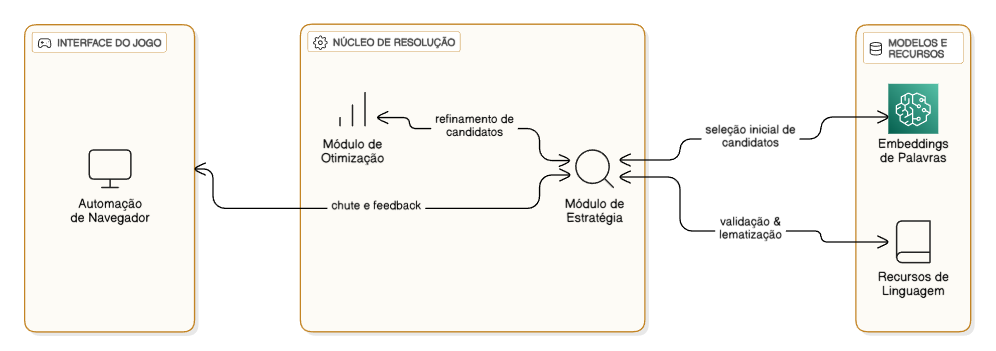
\includegraphics[width=1\textwidth]{figs/diagrama-heuristica.png}
    \label{fig:diagrama-heuristica}
    
    Fonte: Elaborado pelos autores
\end{figure}

\section{Resultados Obtidos}

Esta seção tem como objetivo apresentar e discutir os resultados obtidos durante a execução do algoritmo solucionador desenvolvido, bem como avaliar a eficiência da heurística proposta e o desempenho dos modelos de word embeddings utilizados. O experimento buscou responder três questões centrais: se é possível utilizar word embeddings para resolver jogos de adivinhação de palavras em língua portuguesa; com que frequência o algoritmo é capaz de encontrar a palavra secreta; e por fim, qual modelo apresenta melhor desempenho no jogo Contexto.

\subsection{Metodologia Experimental}

Para garantir a consistência e a reprodução dos resultados, foram conduzidos testes baseado em mil execuções do algoritmo ContextoSolver. Cada execução simulou uma partida do jogo Contexto sendo uma em cada dia do jogo indo do dia um até o dia mil, com limite de cem tentativas para encontrar a palavra-alvo por execução.

Os experimentos foram realizados utilizando três modelos de word embeddings pré-treinados em língua portuguesa, todos com vetores de 300 dimensões, sendo eles, GloVe, Word2Vec e FastText, os dois ultimos foram treinados utilizando CBOW respectivamente. E para cada tentativa, o sistema registrou as seguintes informações: se o jogo foi resolvido com sucesso; o número de tentativas até a palavra correta e a melhor posição alcançada em partidas não resolvidas.

Os dados obtidos foram armazenados em arquivos de log e posteriormente analisados por meio de gráficos gerados em Python (pandas e matplotlib), permitindo a comparação quantitativa e visual entre os modelos.

\subsection{Desempenho Geral}

A Figura \ref{fig:percentual_vitorias} apresenta o percentual acumulado de vitórias por jogo obtido ao longo de 1000 execuções, considerando os modelos GloVe, Word2Vec CBOW e FastText CBOW.

\begin{figure}[H]
    \centering
    \caption{Percentual Acumulado de Vitória por Jogo}
    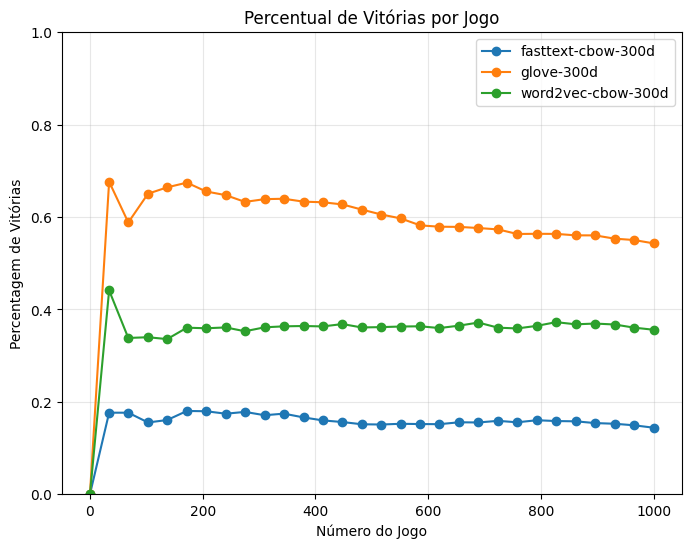
\includegraphics[width=1\textwidth]{figs/percentual_vitorias.png}
    \label{fig:percentual_vitorias}
    
    Fonte: os Autores
\end{figure}

O modelo GloVe obteve o melhor desempenho, obtendo cerca de 54,3\% de vitórias, o que indica maior capacidade em capturar relações semânticas no português. O Word2Vec apresentou desempenho intermediário, com cerca de 35,6\%, menor precisão. Já o FastText teve o pior resultado, com média de 14,4\%, sugerindo que sua ênfase em subpalavras não beneficiou esta tarefa.

De modo geral, o desempenho estabiliza após as primeiras execuções, e o GloVe se destaca como o modelo mais eficaz e consistente para a resolução automática do jogo Contexto em português.

A Figura~\ref{fig:freq} apresenta a distribuição das tentativas realizadas ao longo dos testes analisados na perspectiva do modelo Glove. Observa-se que uma grande parte das partidas foram resolvidas entre 20 e 40 tentativas, evidenciando que o sistema tende a adivinhar a palavra correta após um número moderado de interações com o ambiente. Há, contudo, uma segunda concentração em torno de 75 a 85 tentativas, indicando a existência de partidas de maior complexidade semântica, nas quais as similaridades vetoriais entre a palavra sugerida e o alvo não fornecem indícios suficientemente diretos para a heurística.

Esse comportamento bimodal reflete a variação das palavras propostas pelo jogo. Palavras muito frequentes são mais facilmente resolvidas, enquanto termos com baixa ocorrência no corpus demandam maior exploração. A análise sugere que a heurística implementada é sensível à densidade semântica do espaço vetorial, ajustando-se dinamicamente ao grau de frequência do problema.

\begin{figure}[H]
    \centering
    
    \caption{Distribuição de Tentativas}
    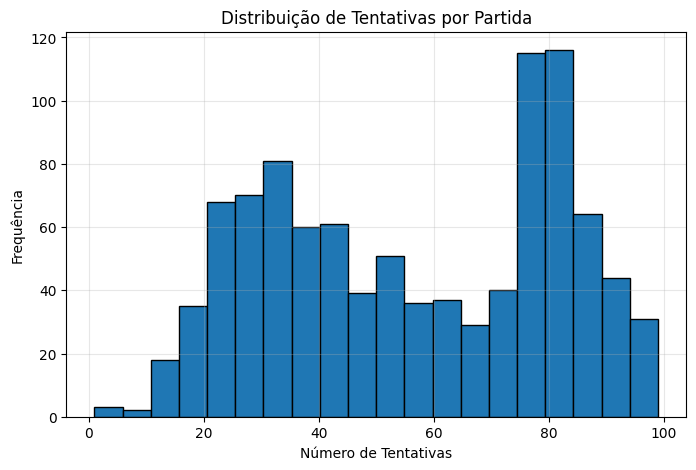
\includegraphics[width=1\textwidth]{figs/freq_vitorias.png}
    \label{fig:freq}
    
    Fonte: os Autores
\end{figure}

\subsection{Síntese dos Resultados}

A partir dos experimentos realizados, é possível confirmar a viabilidade de utilizar word embeddings para resolver jogos de adivinhação de palavras em português, com taxas de sucesso que, em determinados momentos dos testes, superaram 60\% de vitórias. Foi possível identificar que, entre os modelos testados, o GloVe apresentou o melhor equilíbrio entre precisão e consistência, sendo considerado o mais adequado para uso no ContextoSolver.

Além disso, a heurística de resolução desenvolvida se mostrou apropriada e generalizável, permitindo avaliar a qualidade semântica dos modelos de forma consistente.